\chapter{Gestión de Proyectos}

\section{Panel Principal de Proyectos}

Una vez que el usuario ha iniciado sesión, accede a su panel de control o área de trabajo. En esta pantalla se centraliza la gestión de todos los proyectos creados. Un proyecto agrupa todos los modelos, configuraciones y elementos necesarios para definir sintetizadores de audio utilizando el lenguaje de dominio.

\begin{figure}[!ht]
    \centering
    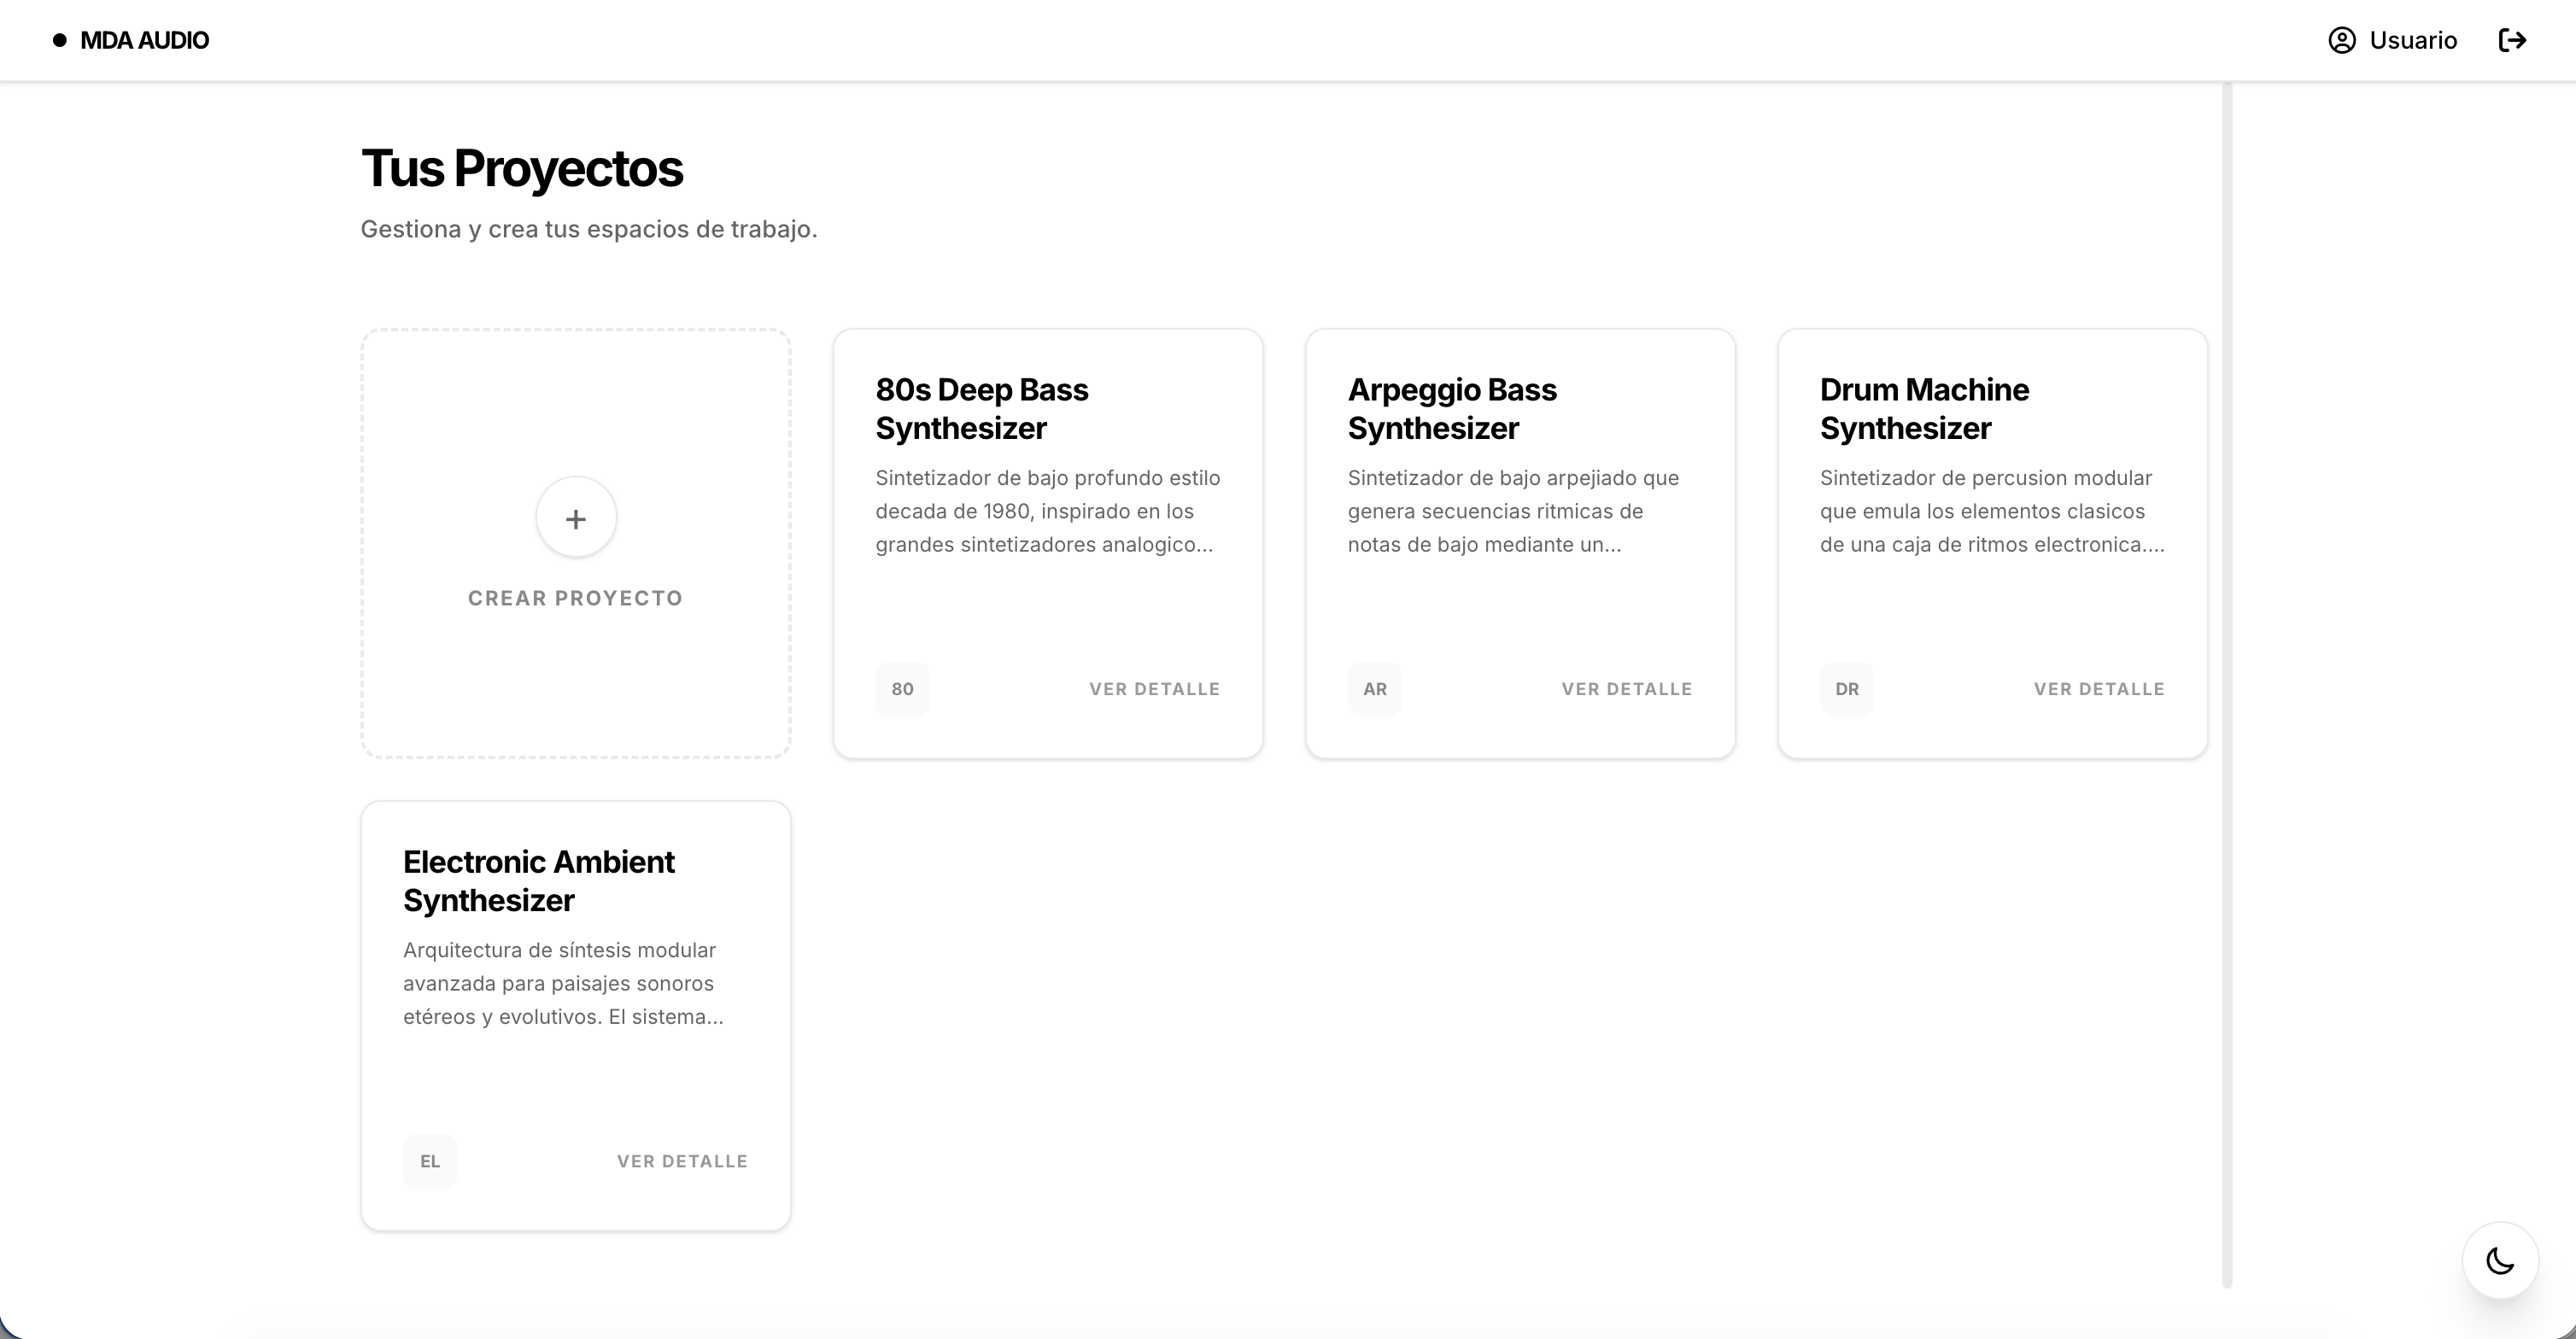
\includegraphics[width=\textwidth]{imagenes/03_proyecto/01_vistaPrincipalConLosProyectos.png}
    \caption{Vista principal con el listado de proyectos.}
\end{figure}

El panel principal ofrece las siguientes capacidades:
\begin{itemize}
    \item \textbf{Visualización de Proyectos:} Cada proyecto se muestra como una tarjeta que incluye su nombre, un color identificativo y un resumen de su contenido o estado.
    \item \textbf{Creación de Nuevos Proyectos:} Botón dedicado para añadir un nuevo elemento al espacio de trabajo.
    \item \textbf{Gestión de la Sesión:} Controles de usuario situados en la barra superior.
\end{itemize}

\subsection{Creación de un Proyecto}

\begin{figure}[!ht]
    \centering
    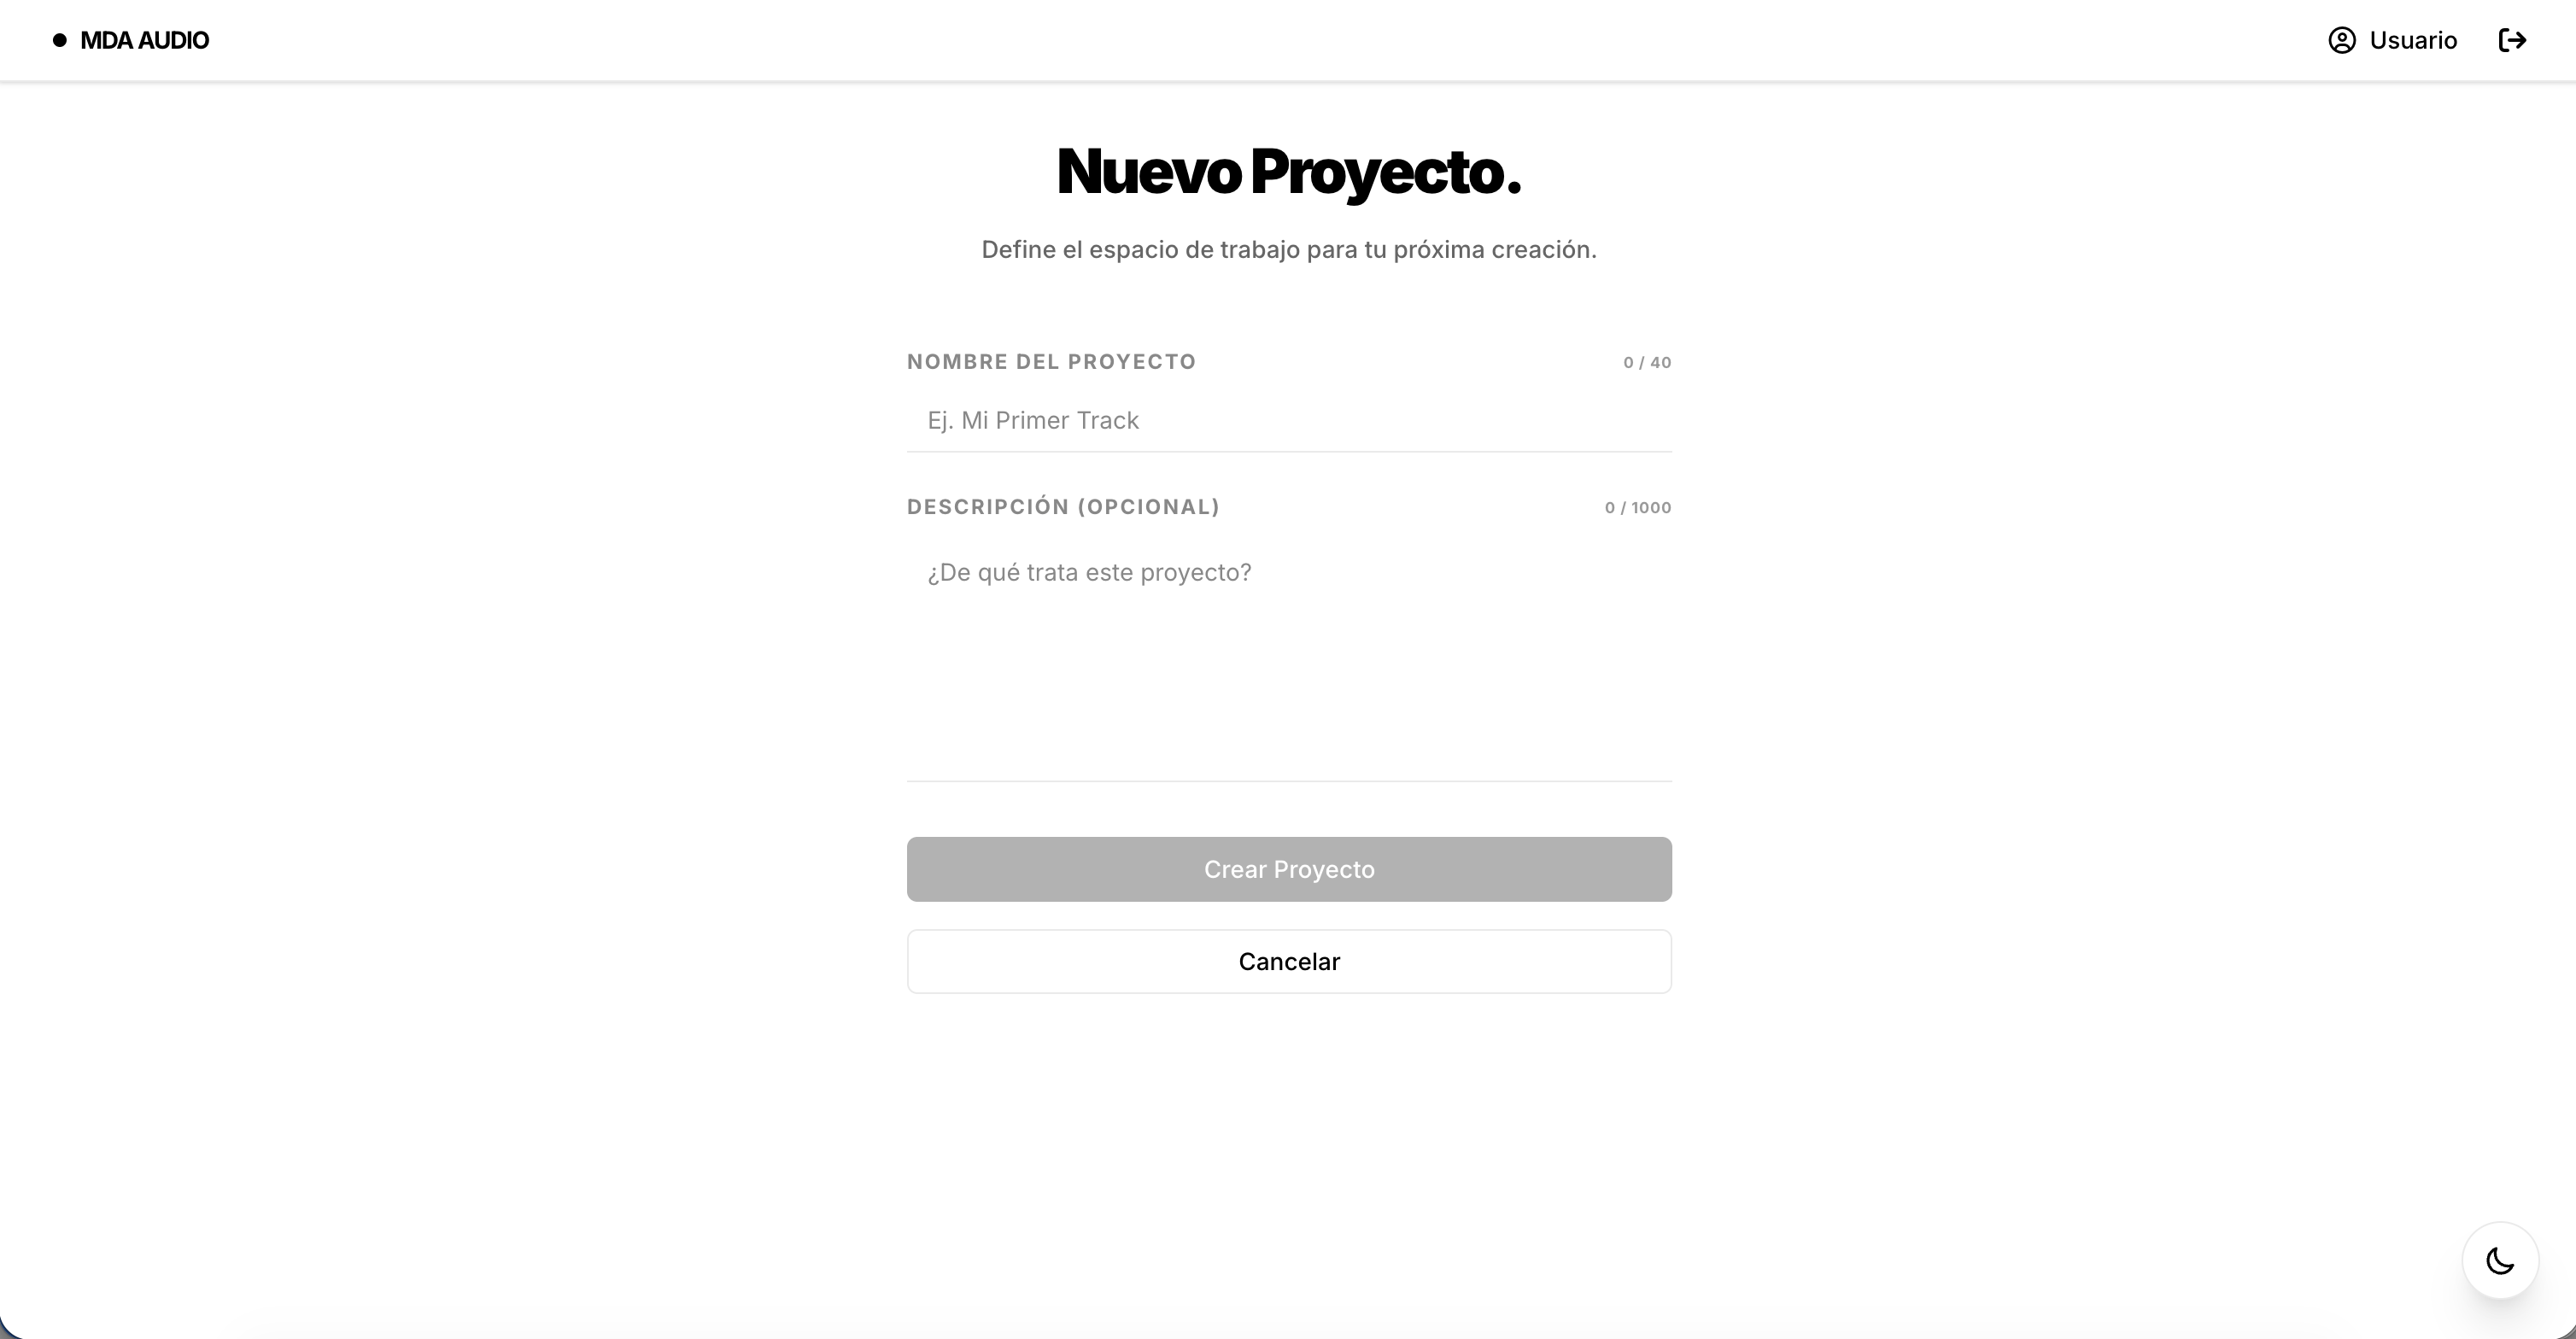
\includegraphics[width=0.6\textwidth]{imagenes/03_proyecto/02_AlPulsarNuevoProyecto.png}
    \caption{Formulario inicial al pulsar nuevo proyecto.}
\end{figure}

Al accionar la opción de crear un nuevo proyecto, se despliega un formulario. Este paso es fundamental, ya que define los metadatos básicos que identificarán al proyecto en el entorno.

\begin{figure}[!ht]
    \centering
    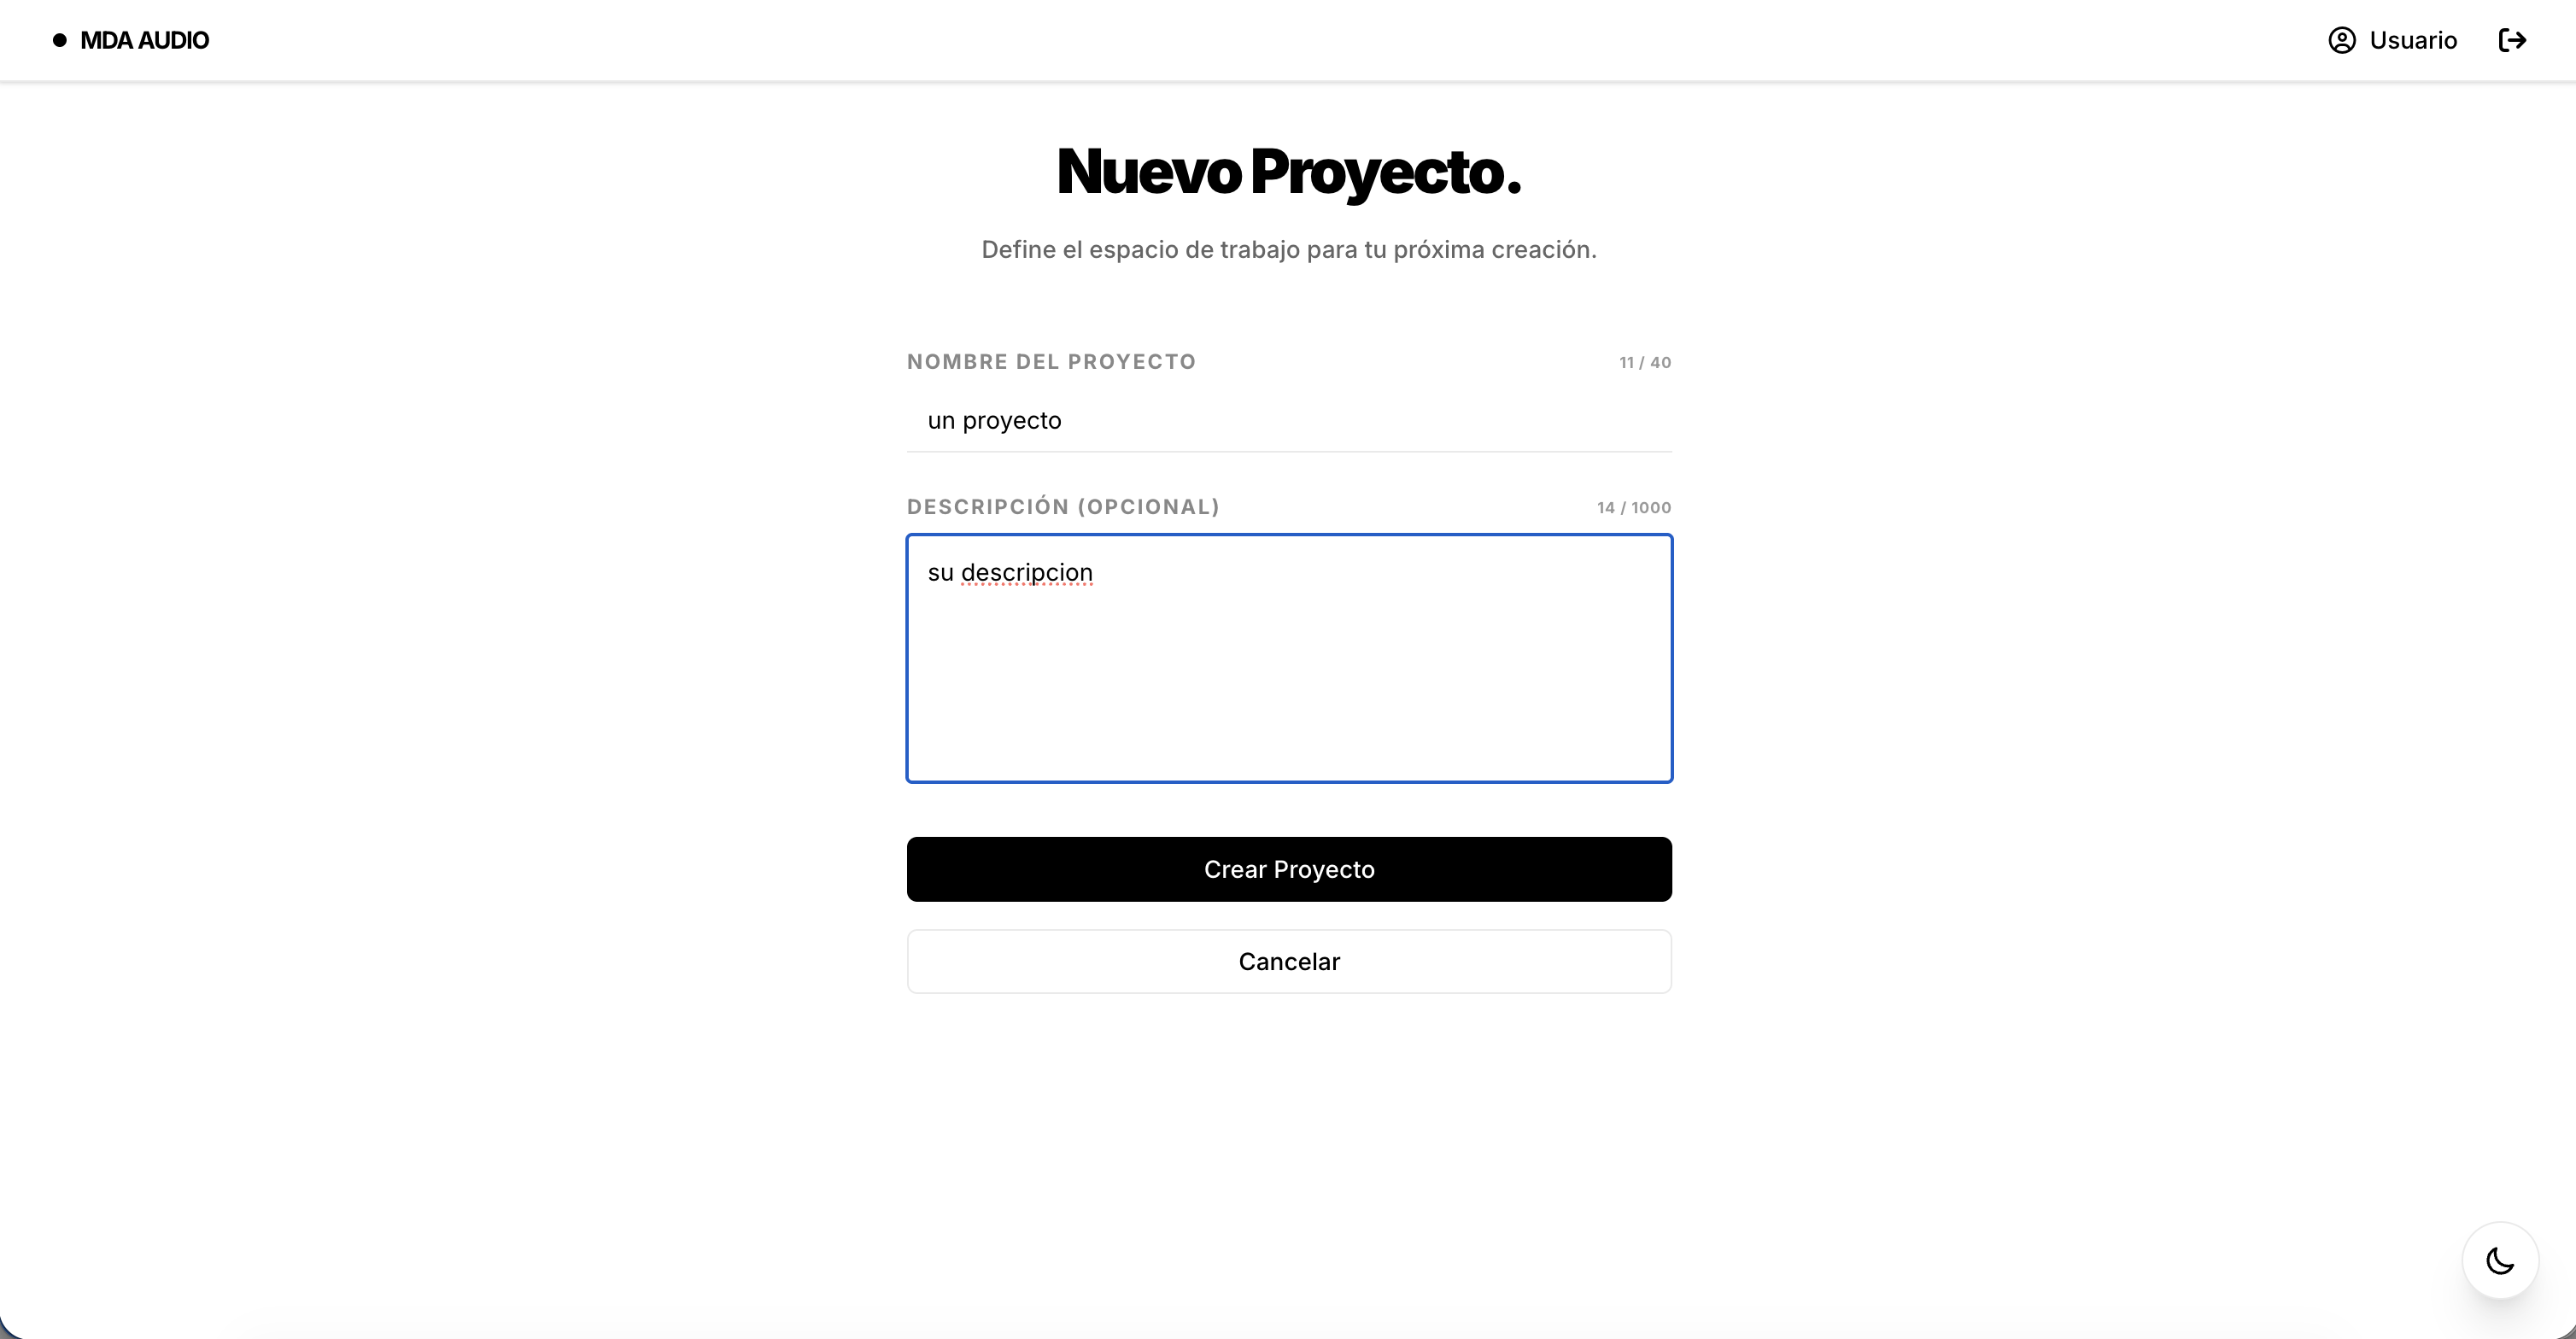
\includegraphics[width=0.6\textwidth]{imagenes/03_proyecto/03_rellenarInformacionNuevoProyecto.png}
    \caption{Relleno de información básica del nuevo proyecto.}
\end{figure}

El usuario debe completar la siguiente información:
\begin{itemize}
    \item \textbf{Nombre del proyecto:} Título descriptivo (ej. \textit{Sintetizador FM Avanzado}).
    \item \textbf{Descripción:} Detalle opcional sobre la finalidad del proyecto.
    \item \textbf{Color identificativo:} Selección de un color para la tarjeta del proyecto, facilitando su reconocimiento visual.
\end{itemize}

\begin{figure}[!ht]
    \centering
    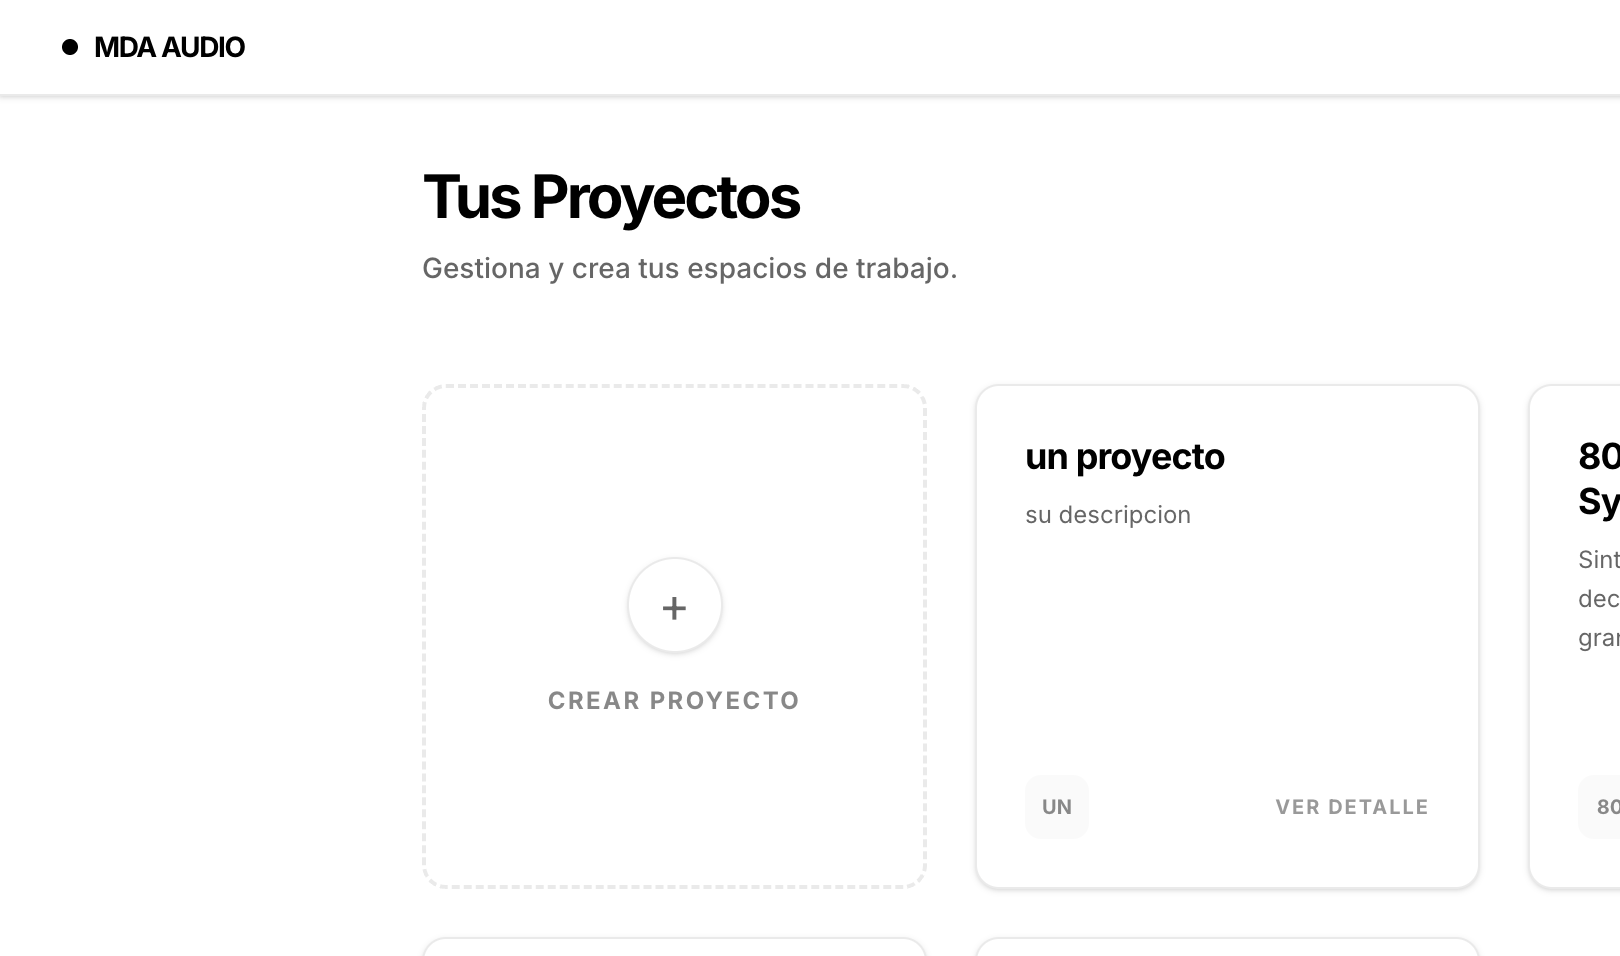
\includegraphics[width=0.6\textwidth]{imagenes/03_proyecto/04_nuevoProyectoCreado.png}
    \caption{Confirmación visual de la creación del proyecto.}
\end{figure}

Tras guardar los cambios, la aplicación confirma la creación y el proyecto aparece inmediatamente en el panel principal como una nueva tarjeta.

\subsection{Modificación y Eliminación}

Las tarjetas de los proyectos en el panel principal ofrecen opciones de gestión rápida sin necesidad de entrar a la edición profunda de modelos.

\begin{figure}[!ht]
    \centering
    
\includegraphics[width=0.4\textwidth]{imagenes/03_proyecto/05_botoneraModificacionYEliminacionProyecto.png}
    \caption{Botonera de opciones en la tarjeta de un proyecto.}
\end{figure}

Cada tarjeta incluye iconos contextuales que despliegan acciones de mantenimiento:
\begin{itemize}
    \item \textbf{Modificar:} Permite editar los metadatos (nombre, descripción, color).
    \item \textbf{Eliminar:} Permite borrar el proyecto y todo su contenido asociado de forma permanente.
\end{itemize}

\begin{figure}[!ht]
    \centering
    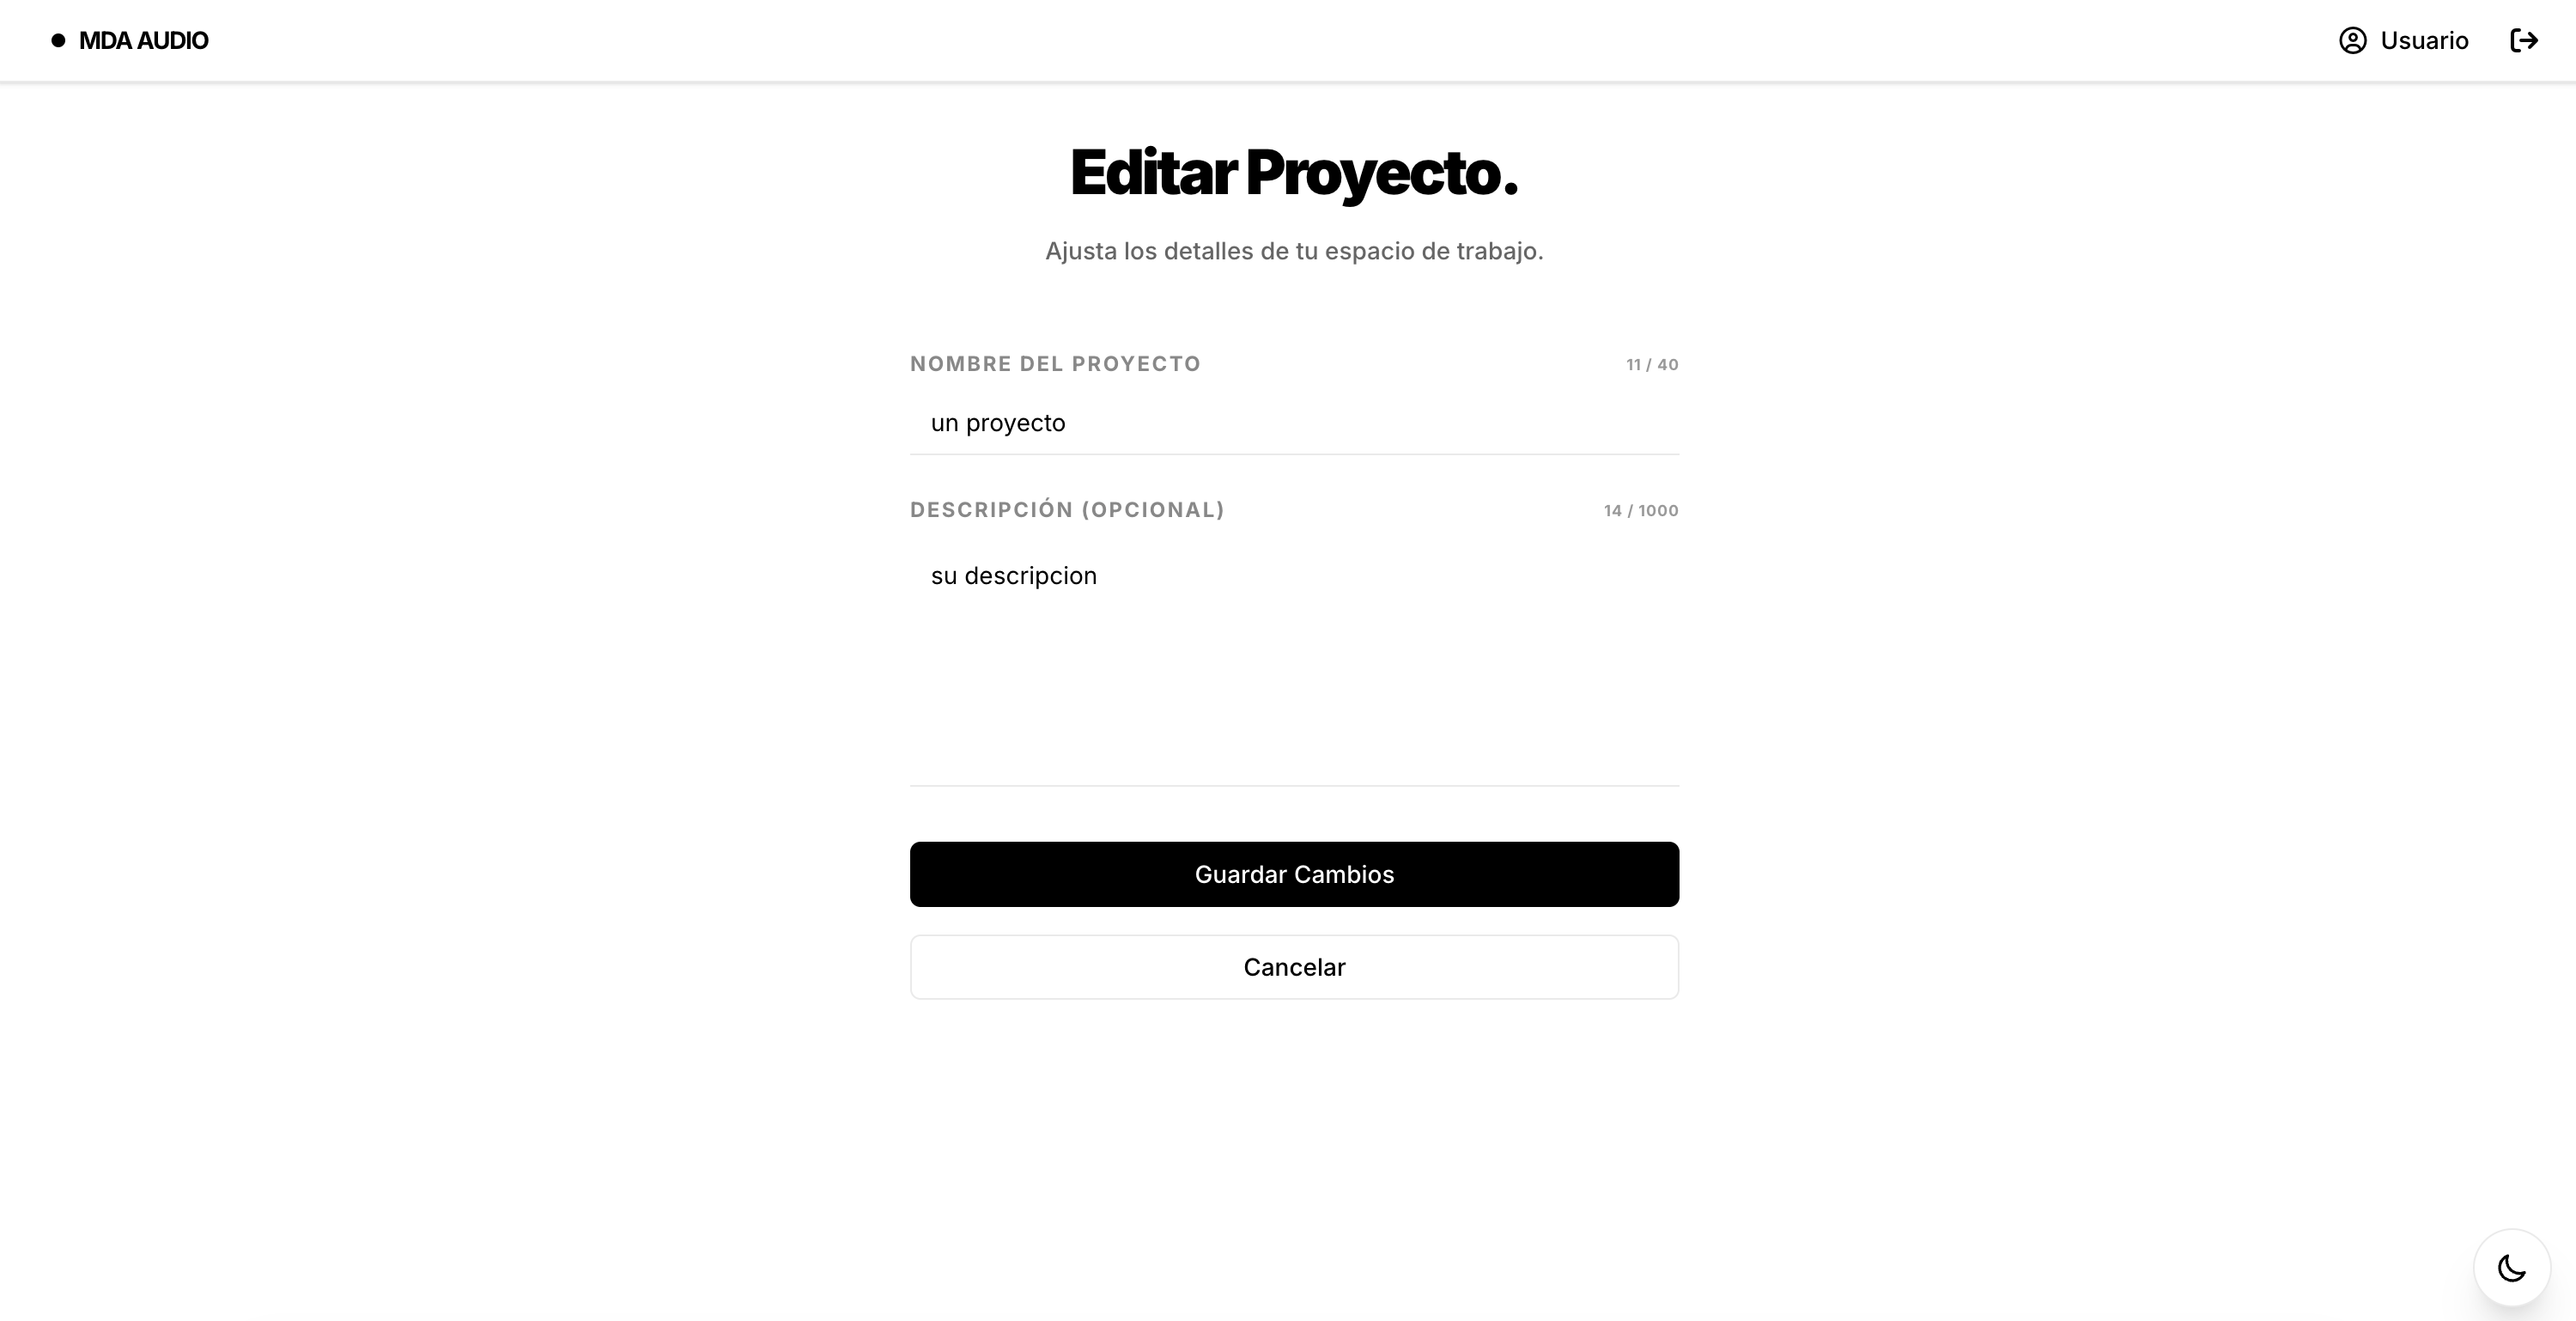
\includegraphics[width=0.6\textwidth]{imagenes/03_proyecto/06_pulsadoBotonModificarProyecto.png}
    \caption{Formulario al pulsar el botón de modificar proyecto.}
\end{figure}

Al seleccionar modificar, se abre el mismo formulario de creación, pero con los datos actuales cargados, permitiendo actualizarlos fácilmente.

\begin{figure}[!ht]
    \centering
    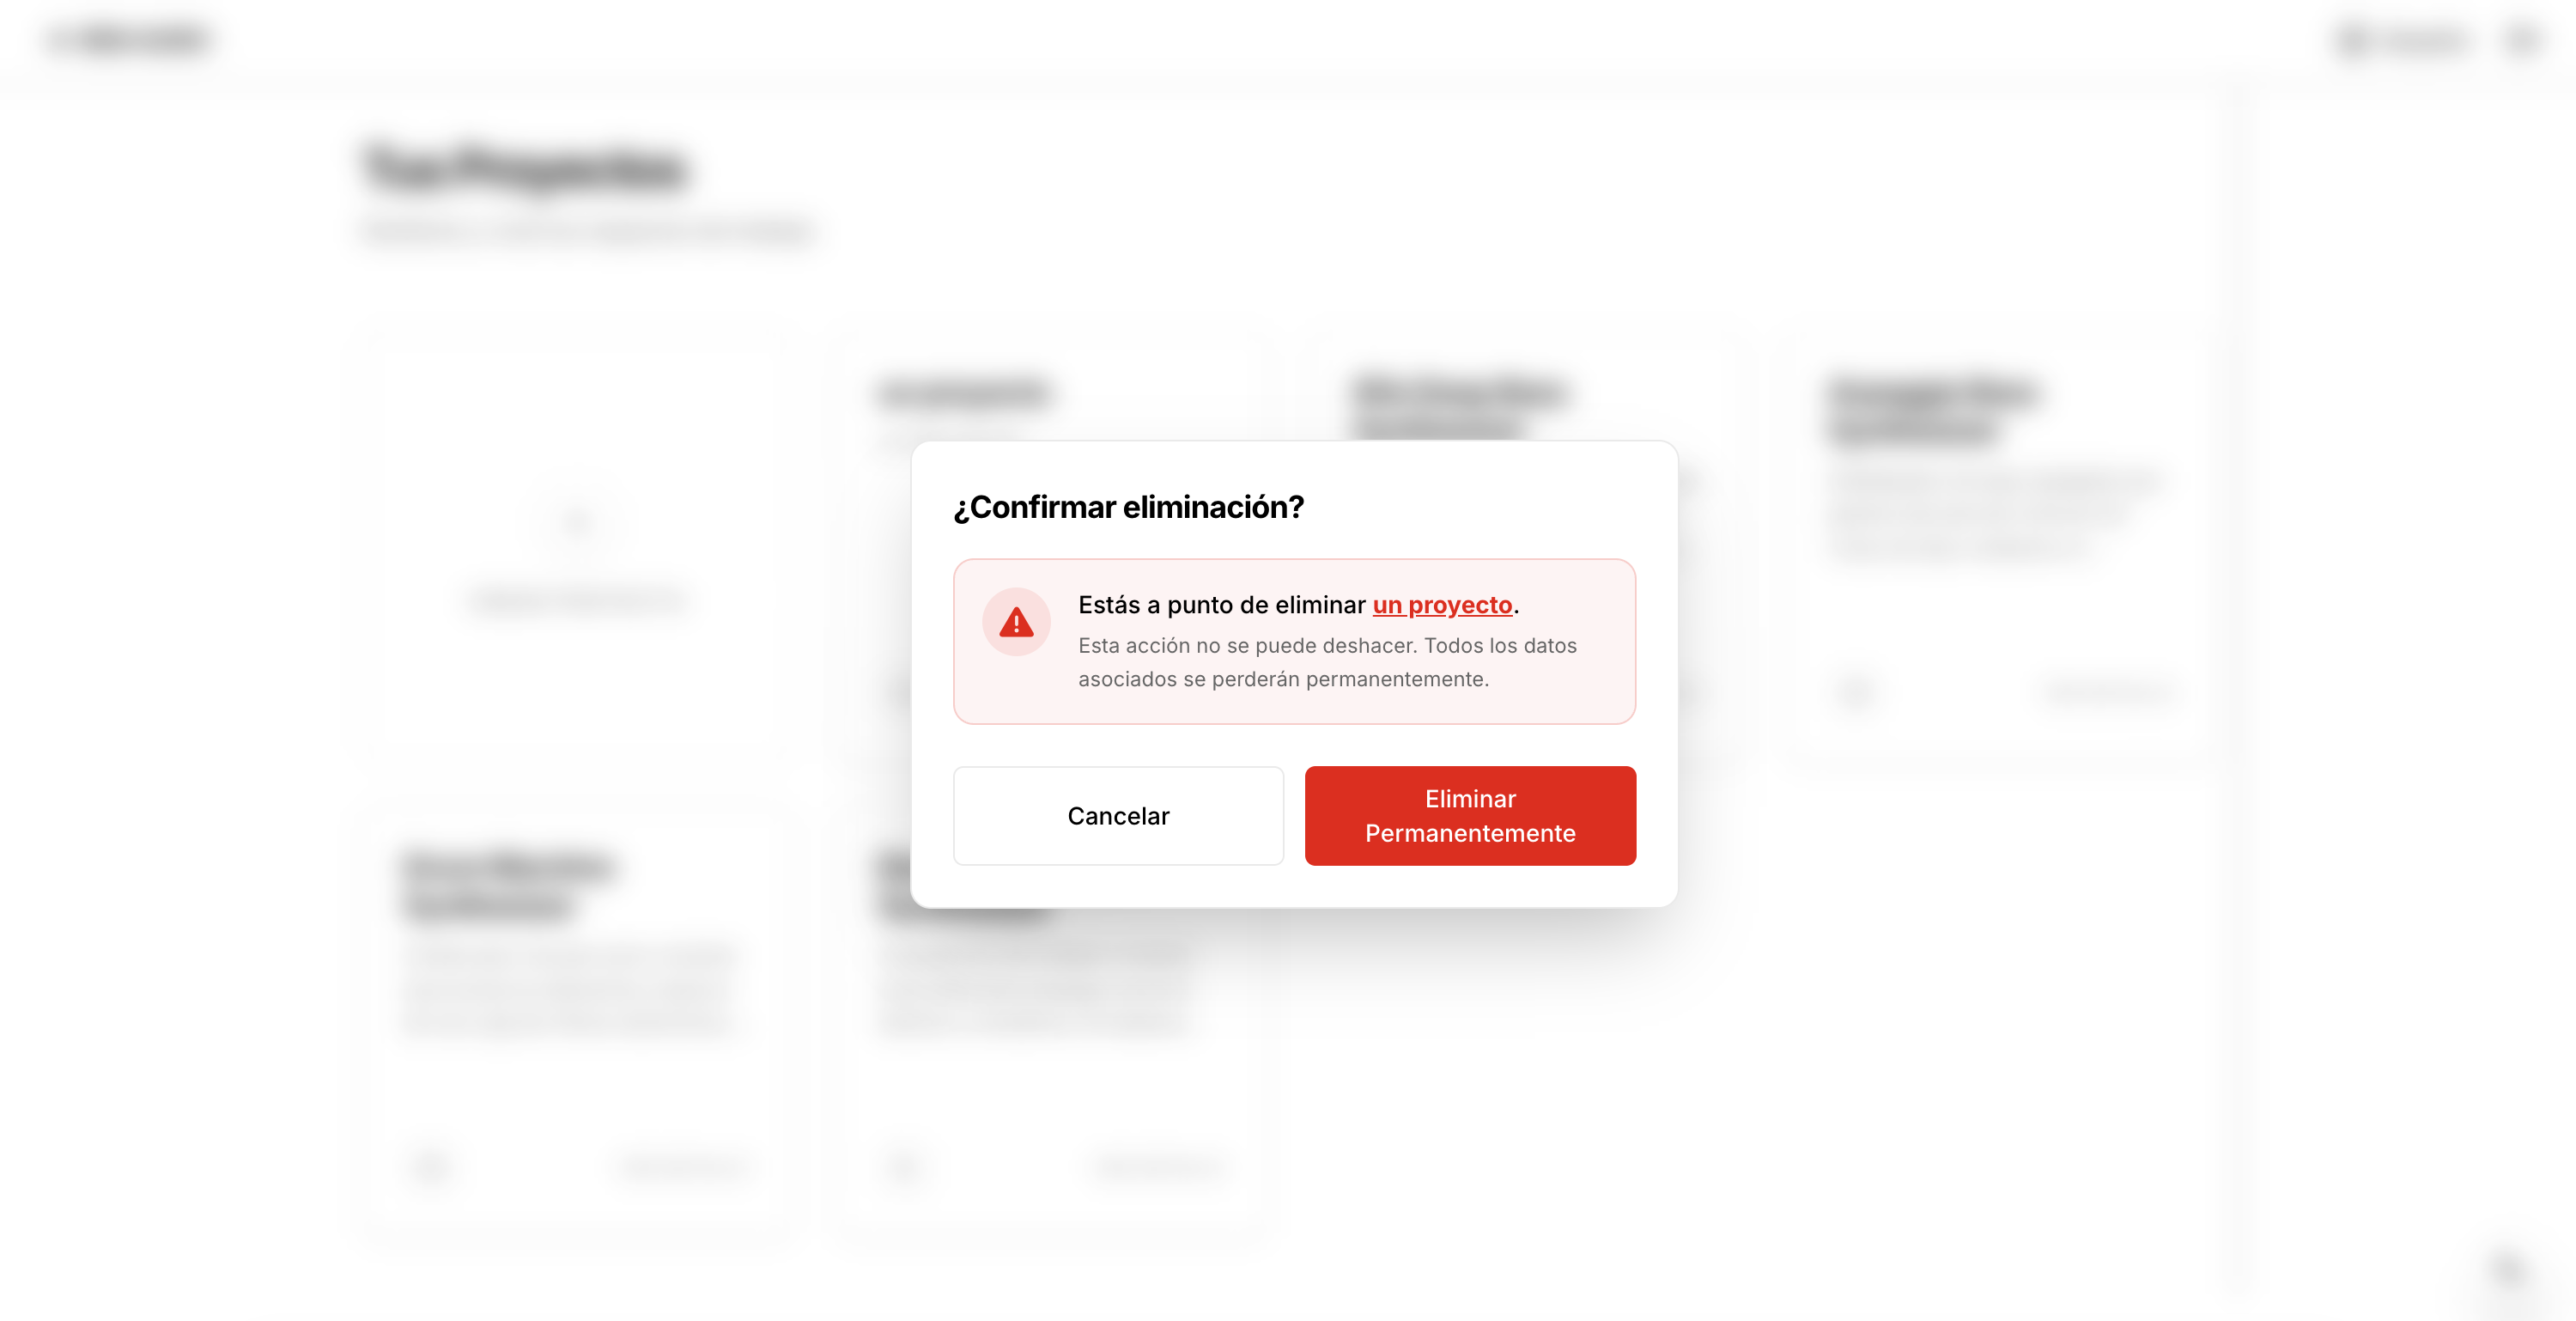
\includegraphics[width=0.6\textwidth]{imagenes/03_proyecto/07_pulsadoBotonEliminarProyecto.png}
    \caption{Aviso de confirmación al eliminar un proyecto.}
\end{figure}

La opción de eliminar es destructiva. Por ello, el sistema siempre solicita una confirmación explícita para evitar pérdidas de trabajo accidentales. Una vez confirmado, el proyecto y sus definiciones en lenguajes \textit{DSL} son eliminados irreversiblemente.

\subsection{Acceso al Espacio de Trabajo del Proyecto}

Para empezar a modelar y definir la lógica musical y el diseño conceptual, el usuario debe abrir el proyecto.

\begin{figure}[!ht]
    \centering
    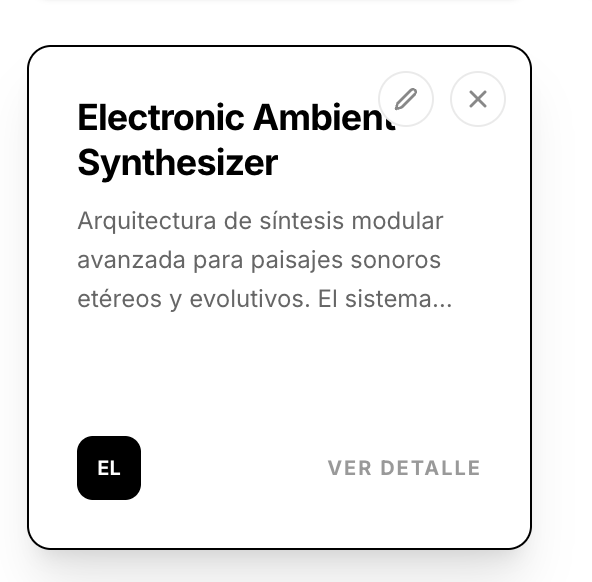
\includegraphics[width=0.6\textwidth]{imagenes/03_proyecto/08_vistaContenidoCajaDeUnProyectoParaPulsarYAbrir.png}
    \caption{Área clicable de la tarjeta para abrir el proyecto.}
\end{figure}

Haciendo clic sobre cualquier parte del contenido de la tarjeta del proyecto (fuera de los botones de modificar/eliminar), el sistema navega al espacio de trabajo específico de dicho proyecto.

\begin{figure}[!ht]
    \centering
    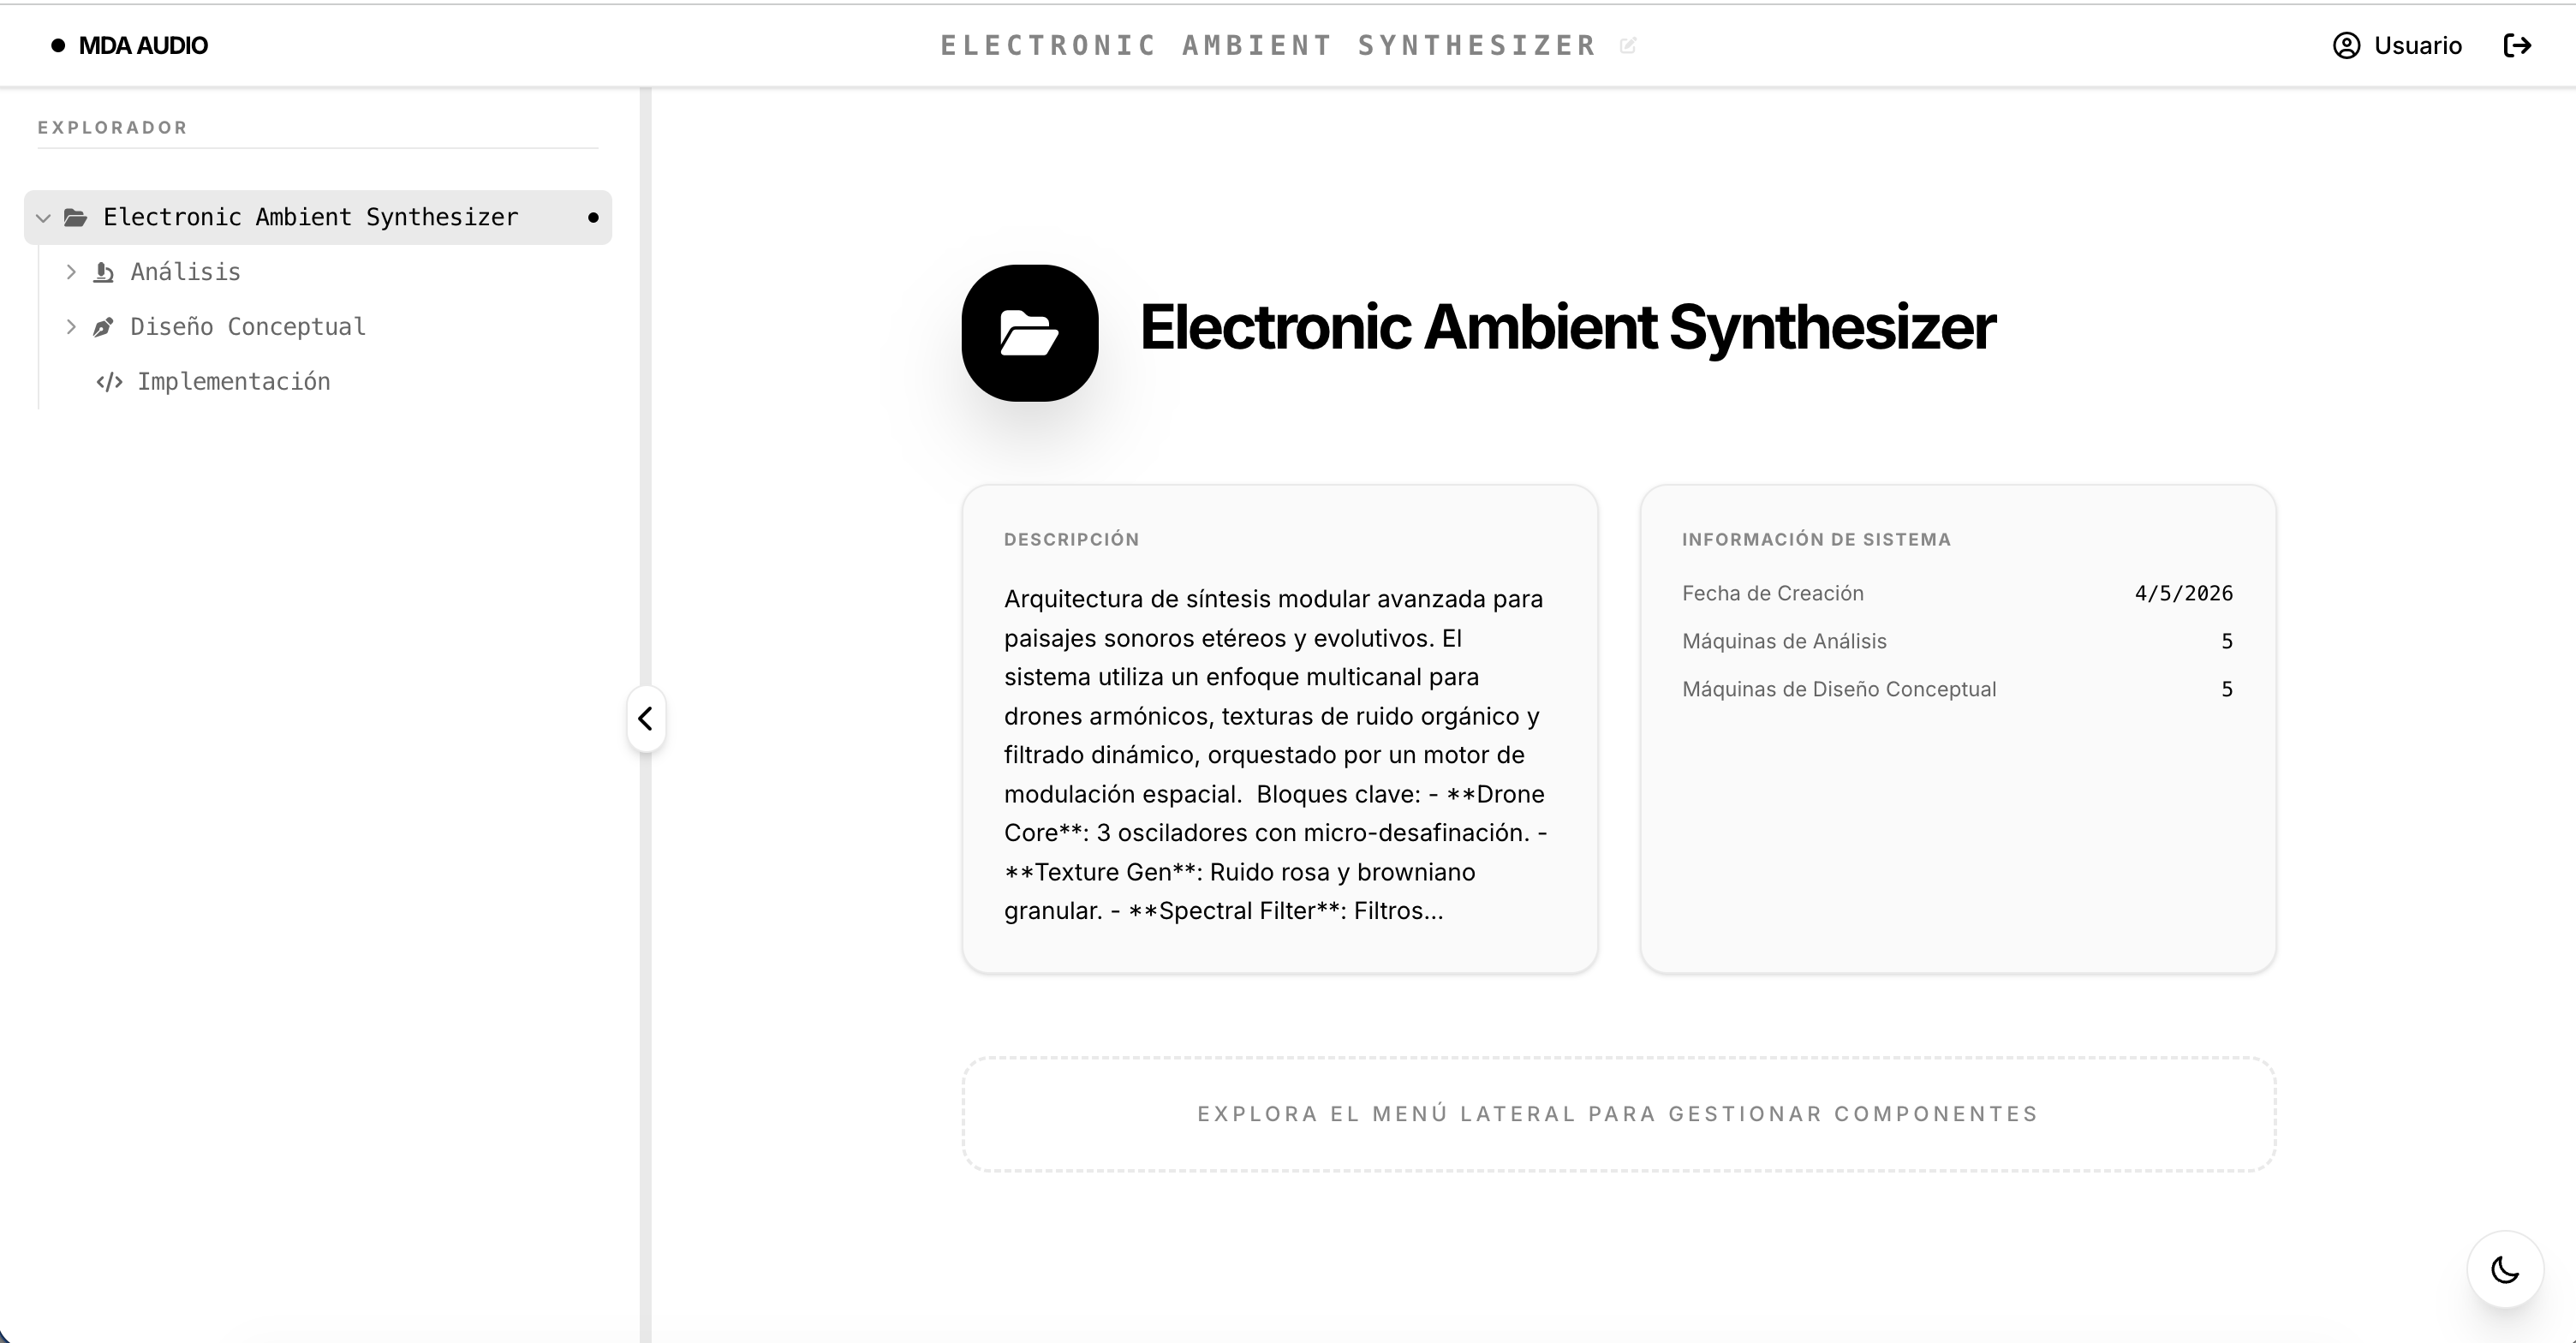
\includegraphics[width=\textwidth]{imagenes/03_proyecto/09_pantallaPrincipalDeProyectoAbierto.png}
    \caption{Pantalla principal tras abrir un proyecto.}
\end{figure}

Dentro de esta pantalla se encuentra el entorno central de la aplicación \textit{MDAA}. Desde aquí se gestionan los modelos independientes de computación (\textit{CIM}) y de plataforma (\textit{PIM}). El proyecto abierto permite también modificar su información básica desde esta misma vista.

\begin{figure}[!ht]
    \centering
    
\includegraphics[width=0.4\textwidth]{imagenes/03_proyecto/10_botonModificarInfoBasicaProyectoDentroPantallaProyecto.png}
    \caption{Botón para modificar información básica dentro del proyecto.}
\end{figure}

\begin{figure}[!ht]
    \centering
    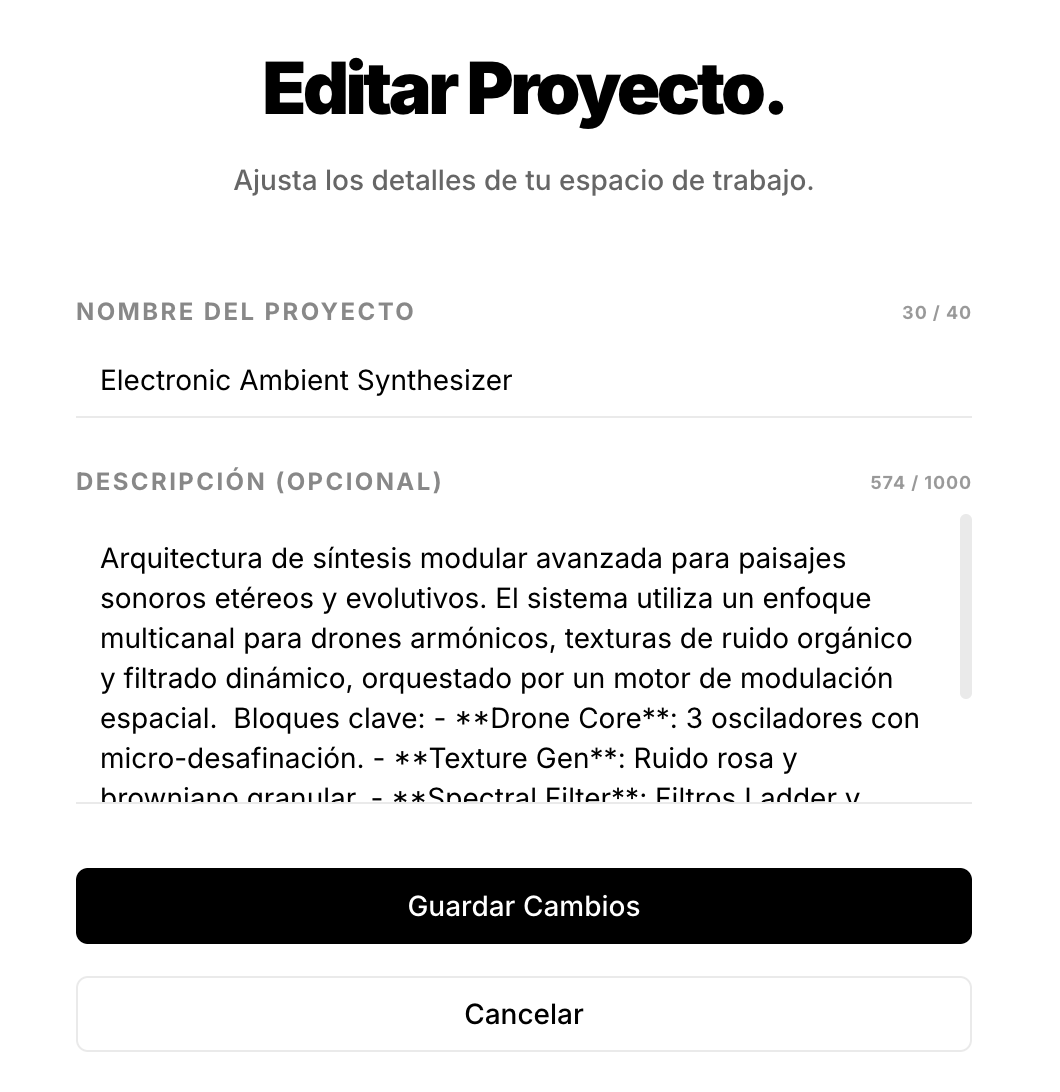
\includegraphics[width=0.6\textwidth]{imagenes/03_proyecto/11_pantallaModificarInfoBasicaProyecto.png}
    \caption{Pantalla de modificación de información básica desde el interior del proyecto.}
\end{figure}

Este botón despliega nuevamente el formulario de metadatos, garantizando que el usuario pueda ajustar el nombre o descripción sin necesidad de regresar al panel principal.

\section{Gestión de Cuenta y Sesión}

Desde el panel principal y cualquier otra vista global, la aplicación ofrece controles de sesión de usuario en la esquina superior derecha.

\begin{figure}[!ht]
    \centering
    
\includegraphics[width=0.4\textwidth]{imagenes/03_proyecto/12_botoneraGestionUsuarioDentroPantallaPrincipal.png}
    \caption{Botonera de gestión de usuario en la barra de navegación superior.}
\end{figure}

\begin{figure}[H]
    \centering
    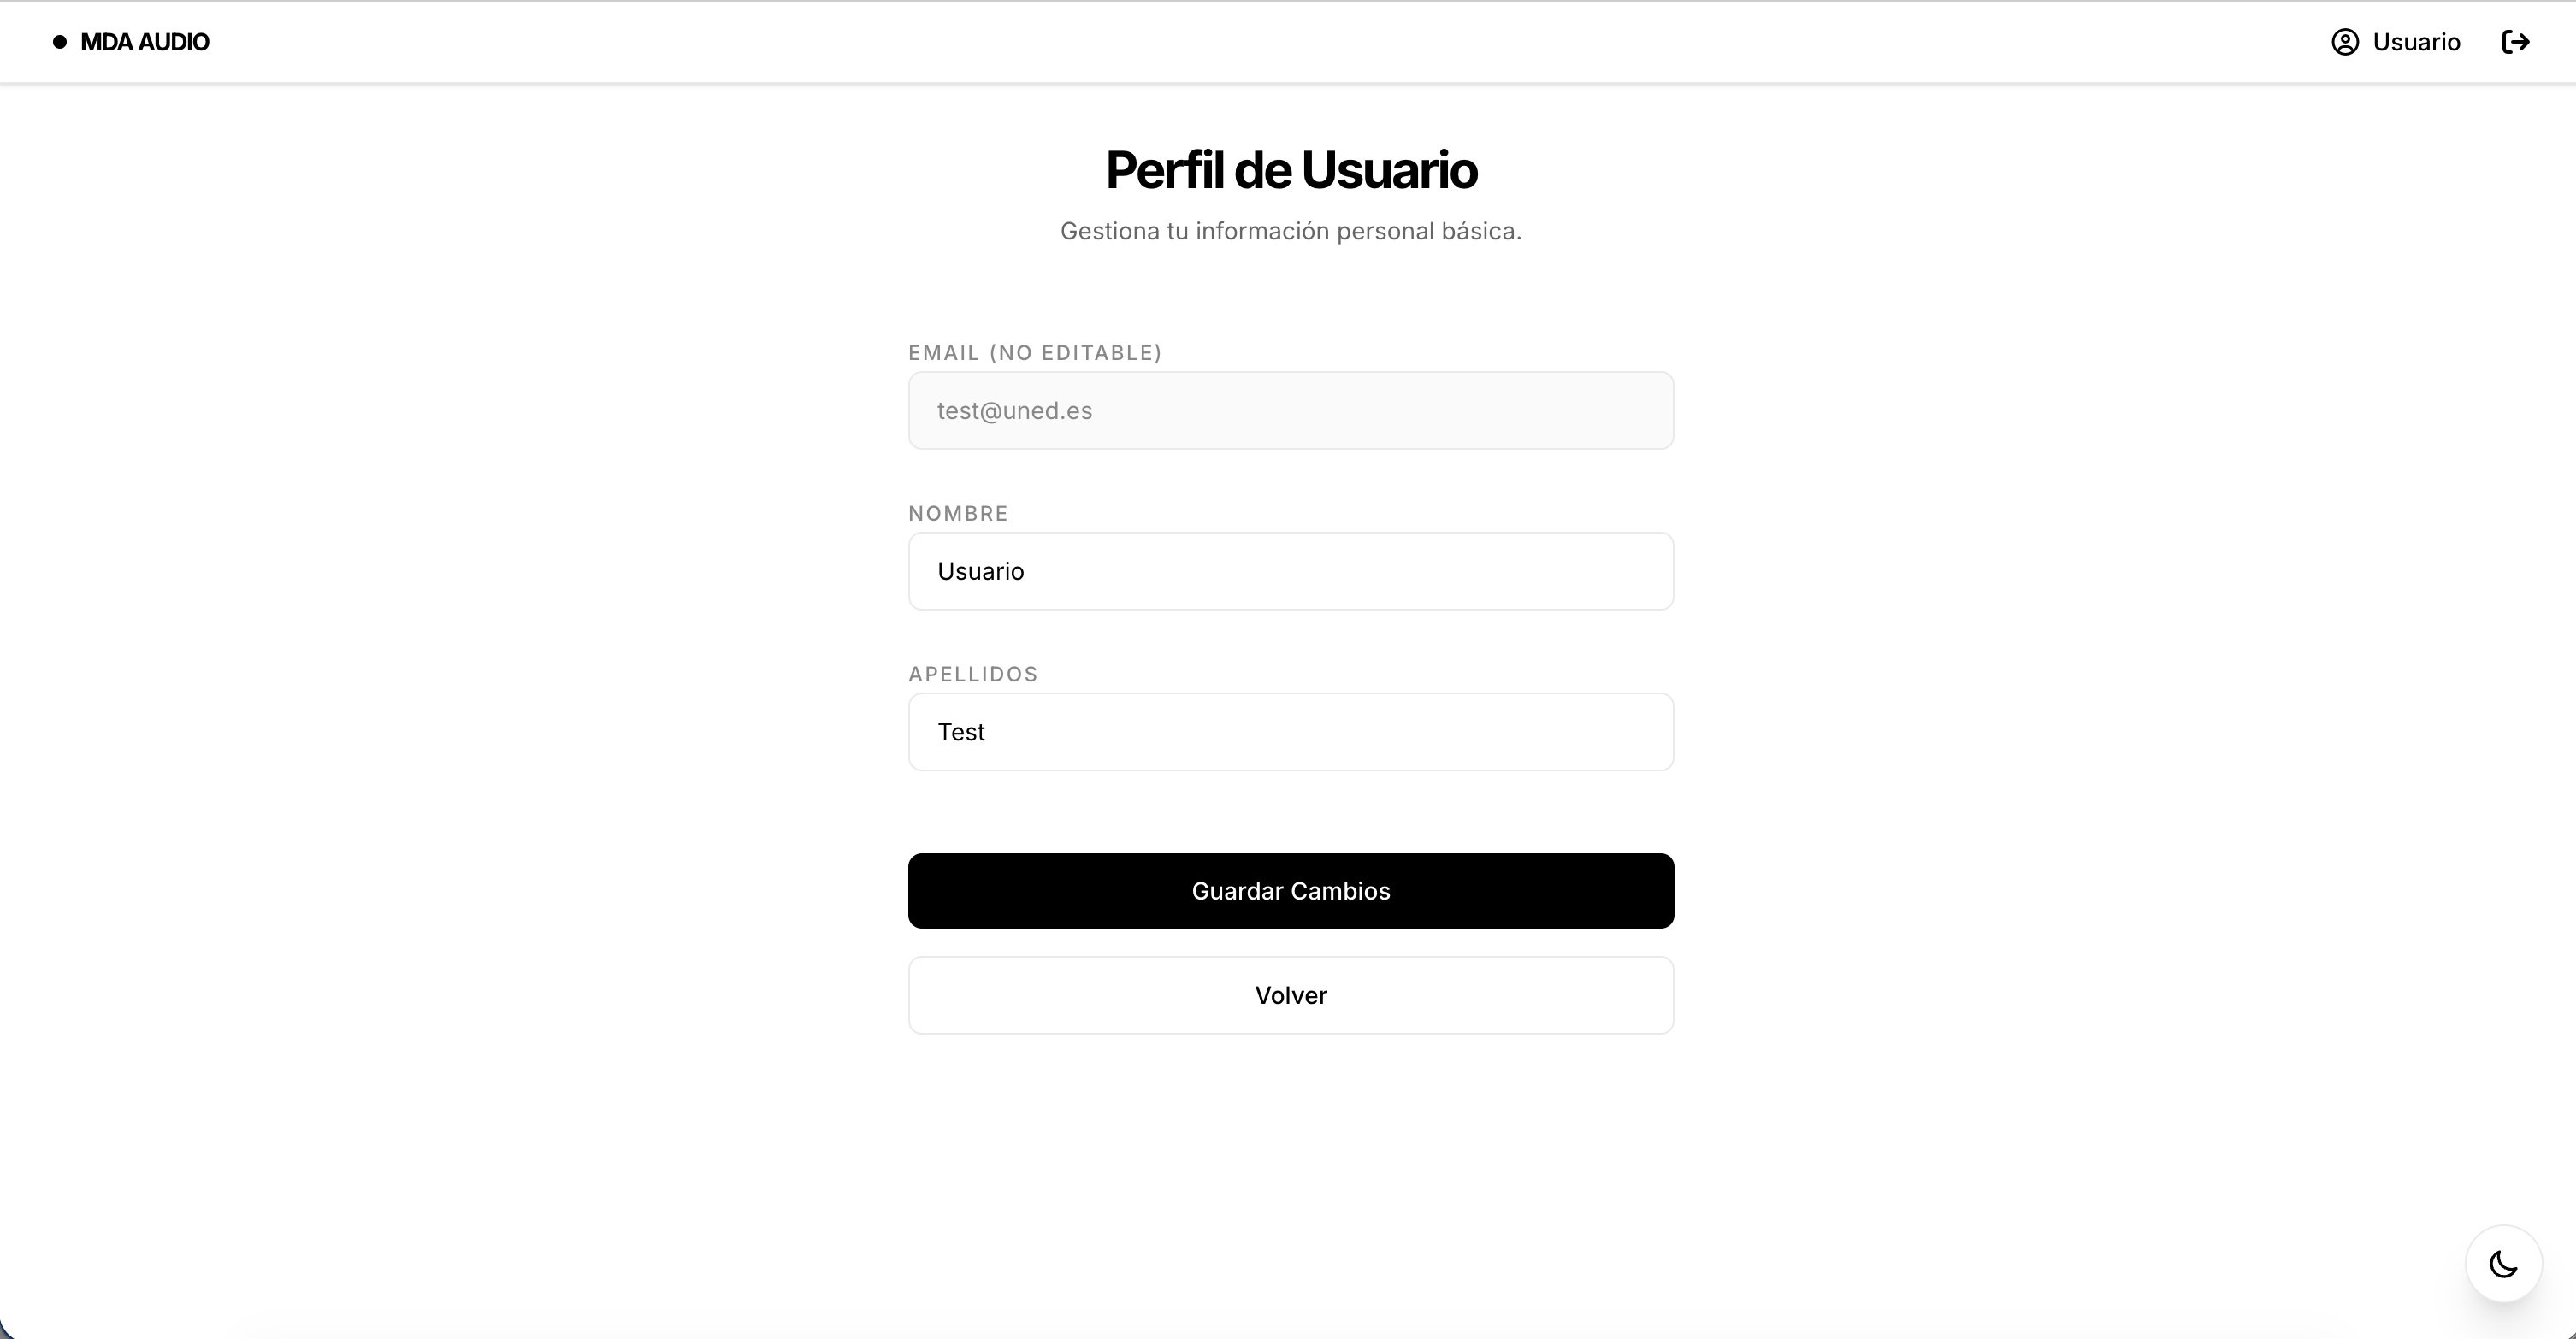
\includegraphics[width=0.5\textwidth]{imagenes/03_proyecto/14_botonUsuarioPulsadoDeGestionUsuarioEnPantallaPrincipal.png}
    \caption{Menú desplegable del usuario.}
\end{figure}

Al pulsar sobre el nombre o icono del usuario, se despliega un menú que incluye:
\begin{itemize}
    \item \textbf{Cerrar Sesión:} Permite salir de forma segura de la aplicación.
\end{itemize}

\begin{figure}[H]
    \centering
    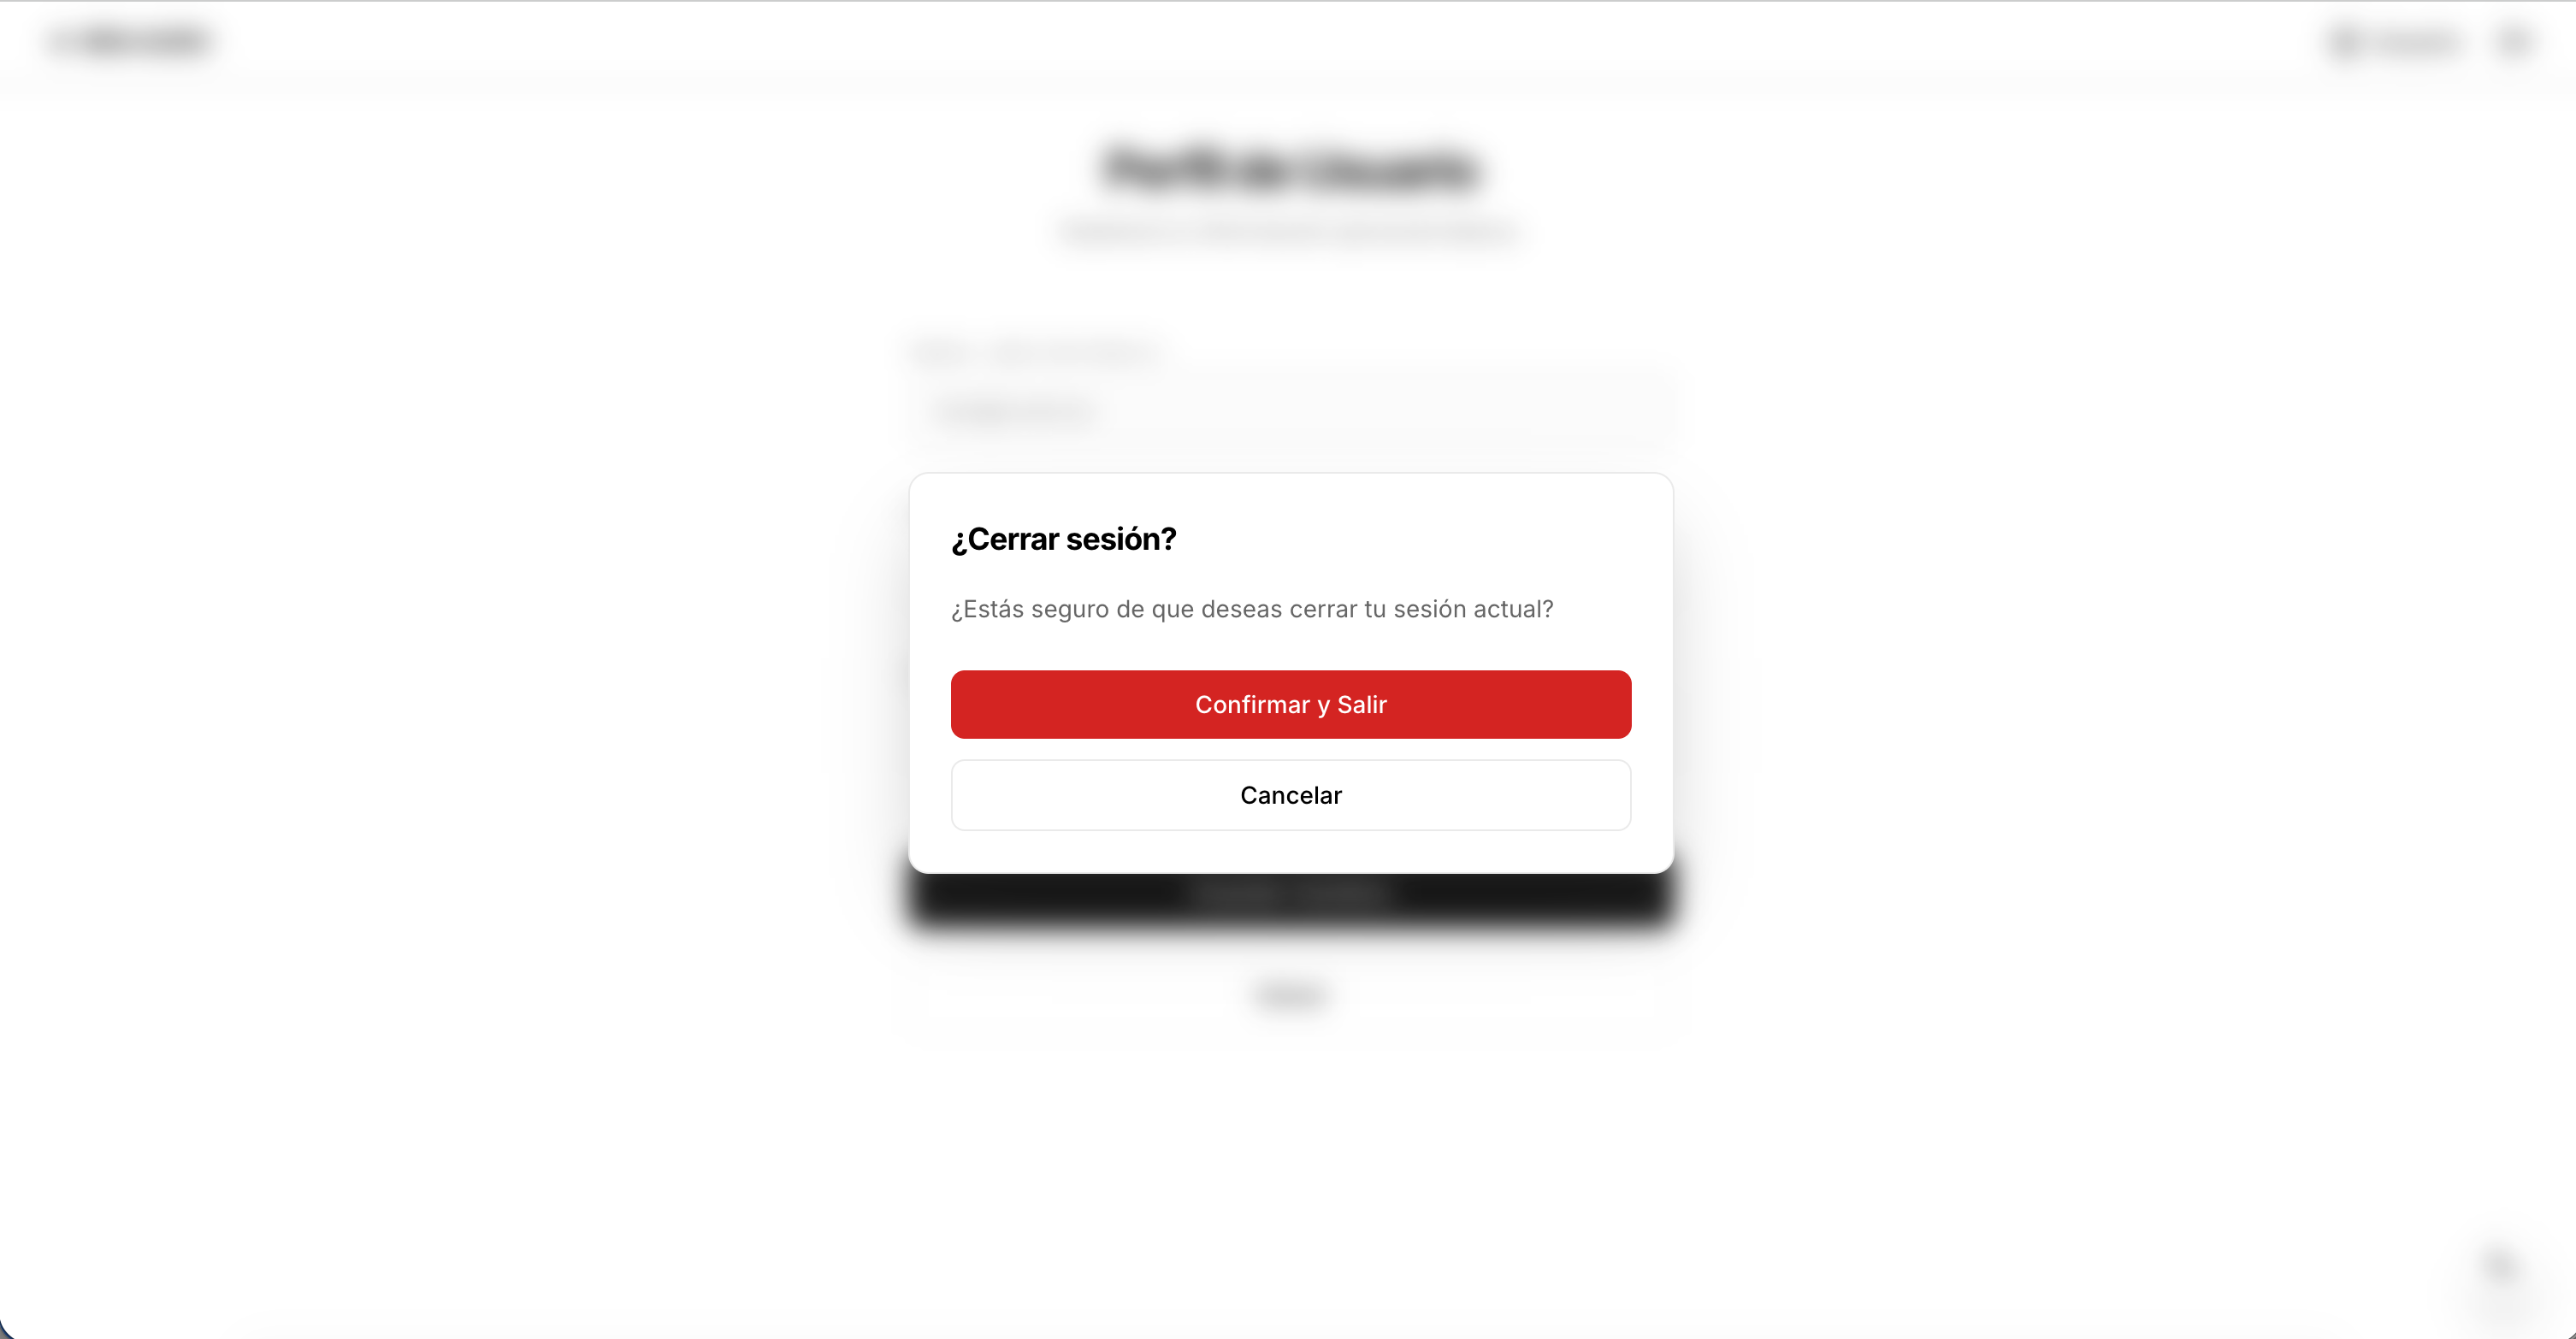
\includegraphics[width=0.6\textwidth]{imagenes/03_proyecto/13_botonCerrarSesionPulsado.png}
    \caption{Aviso de confirmación para cerrar sesión.}
\end{figure}

El sistema solicita confirmación antes de cerrar la sesión, redirigiendo posteriormente a la pantalla de inicio principal.

\begin{figure}[H]
    \centering
    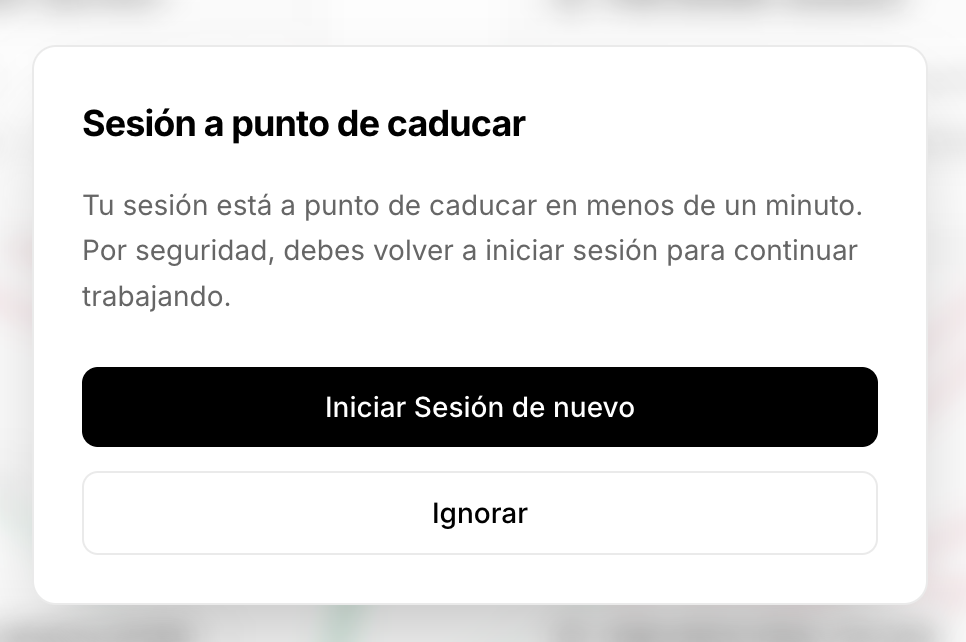
\includegraphics[width=0.6\textwidth]{imagenes/03_proyecto/15_sesionAPuntoDeCaducar.png}
    \caption{Aviso de seguridad por sesión próxima a caducar.}
\end{figure}

Por motivos de seguridad, la sesión tiene un tiempo de expiración. Cuando la sesión está a punto de caducar por inactividad, la aplicación muestra una advertencia, permitiendo al usuario extenderla o dejar que expire, tras lo cual deberá volver a introducir sus credenciales.
